% THIS IS SIGPROC-SP.TEX - VERSION 3.1
% WORKS WITH V3.2SP OF ACM_PROC_ARTICLE-SP.CLS
% APRIL 2009
%
% It is an example file showing how to use the 'acm_proc_article-sp.cls' V3.2SP
% LaTeX2e document class file for Conference Proceedings submissions.
% ----------------------------------------------------------------------------------------------------------------
% This .tex file (and associated .cls V3.2SP) *DOES NOT* produce:
%       1) The Permission Statement
%       2) The Conference (location) Info information
%       3) The Copyright Line with ACM data
%       4) Page numbering
% ---------------------------------------------------------------------------------------------------------------
% It is an example which *does* use the .bib file (from which the .bbl file
% is produced).
% REMEMBER HOWEVER: After having produced the .bbl file,
% and prior to final submission,
% you need to 'insert'  your .bbl file into your source .tex file so as to provide
% ONE 'self-contained' source file.
%
% Questions regarding SIGS should be sent to
% Adrienne Griscti ---> griscti@acm.org
%
% Questions/suggestions regarding the guidelines, .tex and .cls files, etc. to
% Gerald Murray ---> murray@hq.acm.org
%
% For tracking purposes - this is V3.1SP - APRIL 2009

\documentclass{acm_proc_article-sp}

\usepackage{graphicx}
\usepackage{epsfig}
%% The amssymb package provides various useful mathematical symbols
\usepackage{amssymb}
\usepackage{amsmath}
\usepackage{url}
%\usepackage[colorinlistoftodos]{todonotes}

\newcommand{\mytodo}[1]{\textbf{[[#1]]}}
\newcommand{\pseudosection}[1]{\vspace{0.5\baselineskip} \noindent {\bf #1}}

\begin{document}

\title{Hackademics: A Case for Game Jams At Academic Conferences}

\conferenceinfo{Foundations of Digital Games}{2015 Asilomar Conference Grounds, California USA}
%
% You need the command \numberofauthors to handle the 'placement
% and alignment' of the authors beneath the title.
%
% For aesthetic reasons, we recommend 'three authors at a time'
% i.e. three 'name/affiliation blocks' be placed beneath the title.
%
% NOTE: You are NOT restricted in how many 'rows' of
% "name/affiliations" may appear. We just ask that you restrict
% the number of 'columns' to three.
%
% Because of the available 'opening page real-estate'
% we ask you to refrain from putting more than six authors
% (two rows with three columns) beneath the article title.
% More than six makes the first-page appear very cluttered indeed.
%
% Use the \alignauthor commands to handle the names
% and affiliations for an 'aesthetic maximum' of six authors.
% Add names, affiliations, addresses for
% the seventh etc. author(s) as the argument for the
% \additionalauthors command.
% These 'additional authors' will be output/set for you
% without further effort on your part as the last section in
% the body of your article BEFORE References or any Appendices.


%% the REAL DEAL authors; in order of something
 \numberofauthors{5} %  in this sample file, there are a *total*
 % of EIGHT authors. SIX appear on the 'first-page' (for formatting
 % reasons) and the remaining two appear in the \additionalauthors section.
 %
 \author{
 % You can go ahead and credit any number of authors here,
 % e.g. one 'row of three' or two rows (consisting of one row of three
 % and a second row of one, two or three).
 %
 % The command \alignauthor (no curly braces needed) should
 % precede each author name, affiliation/snail-mail address and
 % e-mail address. Additionally, tag each line of
 % affiliation/address with \affaddr, and tag the
 % e-mail address with \email.
 %
 % 1st. author
 \alignauthor
 Michael Cook\\
        \affaddr{Comp. Creativity Group}\\
        \affaddr{Goldsmiths, Uni. London}\\
        \affaddr{London, UK}\\
        \email{mike@gamesbyangelina.org}
 % 2nd. author
 \alignauthor
 Gillian Smith\\
        \affaddr{Northeastern University }\\
        \affaddr{Playable Innovative Technologies Lab}\\
        \affaddr{Boston, MA, 02115}\\
        \email{gi.smith@neu.edu}
 % 3rd. author
 \alignauthor Tommy Thompson\\
        \affaddr{Department of Computing and Mathematics}\\
        \affaddr{University of Derby}\\
        \affaddr{Derby, UK}\\
        \email{tommy@t2thompson.com}
 \and  % use '\and' if you need 'another row' of author names
 % 4th. author
 \alignauthor Julian Togelius\\
        \affaddr{Department of Computer Science and Engineering}\\
        \affaddr{New York University}\\
        \affaddr{New York, NY 11201}\\
        \email{julian@togelius.com}
 % 5th. author
 \alignauthor Alex Zook\\
        \affaddr{School of Interactive Computing}\\
        \affaddr{Georgia Institute of Technology}\\
        \affaddr{Atlanta, GA}\\
        \email{a.zook@gatech.edu}
 }
% Just remember to make sure that the TOTAL number of authors
% is the number that will appear on the first page PLUS the
% number that will appear in the \additionalauthors section.

\toappear{}
\maketitle
\begin{abstract}
%\mytodo{TODO: I still really don't like the alphabetical author order thing. If we can't think of a better way, maybe https://www.random.org/lists/ or even let LaTeX randomise it :D http://texblog.org/2011/04/19/latex-pseudo-random-number-generator/. - MC}
%\mytodo{An academic colleague also suggested we could credit Dagstuhl or the workgroup as the first author? -MC I don't know how to format in LaTeX but have seen before where people place an affiliation below the title and above the author line. Could do that to signify that this was a Dagstuhl working group? -GS}
Game jams are touted as excellent educational experiences for students in higher education, but rarely seen as a valuable activity for scholarly work.
We argue for incorporating game jams and other hackathon activities into academic conferences and scholarly meetings, due to their abilities to foster interdisciplinary collaboration, ease newcomers into game creation, and promote innovative and experimental game designs.
We reflect on a highly-successful game jam at a recent Dagstuhl Seminar, and make recommendations for how to incorporate game jams into future conferences.
\end{abstract}

% A category with the (minimum) three required fields

\category{Applied Computing}{Computers in other domains}{Personal computers and PC applications}[Computer games]
%\category{H.4}{Information Systems Applications}{Miscellaneous}
%A category including the fourth, optional field follows...
%\category{D.2.8}{Software Engineering}{Metrics}[complexity measures, performance measures]

\terms{Design}

\keywords{Game Jam, Hackathon, Game Design, Interdisciplinarity} % NOT required for Proceedings

%%%%%%%%%%%%%%%%%%%%%%%%%%%%%%%%%%%%%%%%%%%%%%%%%%%%%%

\section{Introduction}
%\mytodo{AZ: any assertions that are too strong + need support?}
Game jams are a catalyst for innovation and creativity.
The focused atmosphere, time and thematic constraints, and opportunity for new collaborations permit participants to explore new game concepts, and give them the time and permission to work on projects they might otherwise think too risky, too time consuming, or too challenging to complete outside of a jam environment~\cite{musil2010:jam-software-dev}.
For these reasons, game jams are often pitched as valuable educational experiences for students: over a hundred Global Game Jam (GGJ) sites were held on university campuses in 2015, a PhD program in the UK has game jam entry as part of its syllabus\footnote{http://www.iggi.org.uk/}, and jams held online are increasingly advertised to students or even integrated into university courses~\cite{cook:procjam}.

%\mytodo{GS: My guess is that the next paragraph is where reviewers wanted citations. But I don't know of anything we can cite, and it seems like relatively common sense...}
%
%\mytodo{T2: Agreed.  I can't think of any formal academic writing that we could cite to remedy that comment.}

Game jams are dynamic and targeted events that encourage teamwork and interdisciplinary collaboration.
These strengths are beneficial for students and can also offer benefits that offset some of the shortcomings of academic research events too.
Academic meetings---conferences, workshops, and symposia---typically involve researchers sharing and critiquing work they have already done on their own, and often fragment their audience or submissions according to research themes or expertise.
Game jams offer an alternative format to remedy these shortcomings: forming interdisciplinary teams of developers, designers, artists, and critics who create something in a short time frame by combining their skills and knowledge in ways that are hard to do with traditional long-term research projects.

We argue that game jams can produce ``playable research'': practical demonstrations of theoretical ideas.
Jams can bypass the long development cycles of huge, multi-site research grants, and relieve justification in terms of money or time.
While the output of a game jam is unlikely to be polished or properly tested, it has the advantage of~\emph{existing}, providing a demonstration to others, evaluated as an early prototype, and potentially written up as further research output.

% academic findings on impact on collaboration/creativity of game jams (Alex)
Game jams also foster individual creativity and learning.
Researchers have found GGJ participants become more familiar with and confident in game development processes~\cite{arya2013:ggj-learn}.
Jam themes help direct people as inspiration and encourage greater creativity~\cite{kultima2011:ggj-creative, zook2013:ggj-conceptualization}.
Jams can encourage novel academic work while benefiting individual participants.
%Our experiences with an AI-based hackathon align and augment these results: we look at a case where the ``theme'' is a mechanic (AI) and where participants have experience in game development, but are working with new teams.
%Studying academic hackathons stands to shed light on how academic professionals benefit from and contribute to hackathons, moving beyond personal benefits such as game development experience or confidence.

We argue for incorporating game jams into academic events.
We contend game jams are useful for the production of new scholarly work, present a case study of a game jam performed at the Dagstuhl Seminar on CI/AI in Games, and provide recommendations for the organization of new academic game jams in the future.
We hope to show that game jams are easy to integrate into existing academic event formats, and can give rise to new and interesting work that we believe would be unlikely to come about any other way.


%However, the benefits of game jams can and should also be brought to bear on academic research. Though there have been some workshops and studios that focus on building things (e.g. the game studies curriculum workshop \textbf{find real name, this is Mia's thing}), the focus of technically-oriented game research is on presenting papers, giving demos, and sharing thoughts on where the field should move in the future. This is a symptom of the culture of competition and focus on individual achievement in academia: researchers compete to get their papers into a conference or journal and then argue their case during presentation. Game jams, on the other hand, encourage collaboration between participants in order Game jams, on the other hand, are highly collaborative, force participants to act as well as theorize, and drive interdisciplinary collaboration.

%%%%%%%%%%%%%%%%%%%%%%%%%%%%%%%%%%%%%%%%%%%%%%%%%%%%%%

%\section{Related Work}

%\mytodo{[AZ] RW mostly felt extraneous/unrelated; now folded into intro}

%% academic findings on impact on collaboration/creativity of game jams (Alex)
%Game jams also foster creativity and learning.
%%Most studies examine general participation in the annual Global Game Jam (GGJ) through surveys or direct observation of participants.
%Arya et al. \cite{arya2013:ggj-learn} surveyed 2012 GGJ participants finding people were became more familiar with and confident in game development processes post-jam compared to pre-jam.
%% [AZ] hate self-citation, but it's an actual survey rather than position piece...
%Zook and Riedl \cite{zook2013:ggj-conceptualization} surveyed 2013 GGJ participants, finding people design games simply to finish making a game, test out a game mechanic, or give players an enjoyable experience.
%People cited the jam theme as their primary source for inspiration, followed by a desired mechanic, other game, or general game genre.
%Kultima and Alha \cite{kultima2011:ggj-creative} found that providing brainstorming tools (specifically their Verbs, Nouns, and Adjectives tool) with a thematic focus can support creativity in game jams.
%Our experiences with an AI-based hackathon align and augment these results: we look at a case where the ``theme'' is a mechanic (AI) and where participants have experience in game development, but are working with new teams.
%Studying academic hackathons stands to shed light on how academic professionals benefit from and contribute to hackathons, moving beyond personal benefits such as game development experience or confidence.



%%%%%%%%%%%%%%%%%%%%%%%%%%%%%%%%%%%%%%%%%%%%%%%%%%%%%%

\section{Why Game Jams in Academia?}
Game jams can benefit scholarly research as a whole, individual participants at the personal and professional levels, and even the established game jam culture.
%\mytodo{either turn this into a long bulleted list, or add connective tissue between each paragraph. Or maybe both.}
Game jams are highly interdisciplinary events, bringing together people from a variety of technical, artistic, and humanistic backgrounds.
For example, at the recent GGJ at Northeastern University, one team consisted of students from an art college, students from a technically-focused degree program, and a faculty member from the School of Law.
Though conferences often aim to promote interdisciplinarity, this primarily occurs by accepting papers from a variety of disciplines and presenting them in disciplinary-focused tracks.
A game jam brings together people from different disciplines to collaborate in an intense and focused environment.
By encouraging participants to build something with members of other disciplines there is great potential for new collaborations and learning from those in other fields.
This comes through combining game development skills (such as artists and designers working with programmers and musicians), combining research expertise, and mixing cutting-edge ideas that would normally never mix.
%TODO I think this is maybe the most important reason. I'm not sure how to better highlight it. Maybe move some of the text about the current way interdisciplinarity is handled at conferences to the intro?

Building games and other playable experiences is a reflective process, allowing the designer(s) to deeply investigate the concepts addressed by the game through the process of making the concepts concrete in the game's design \cite{mateas2001expressive, schon1983reflective}.
%\mytodo{what is collaborative critical making? GS: put in a citation to a critical making workshop outside of games. if we really want to go into it, could also cite Flanagan and Bogost as examples of people who think about different aspects of critical making, but I really don't want to have a long aside on the definition of "critical making" in this paragraph, that's like a paper in itself}
Having academics who often do not create games in their scholarly work participate in game jams creates the opportunity to bring deep domain expertise to the process, and for encouraging critical making in game design in a conference setting (as has been done outside of game design \cite{tanenbaum2014:critical-making}).
While this critical reflection may not occur until after the jam, the shared experiences and products offer the potential to develop scholarly research.
%\mytodo{This might be a hard sell because game jamming typically does not allow the same amount of reflection one might normally get. -MC}

Game jams force consideration of pragmatic concerns: from a game technology perspective, a system that works well in theory or even in the typically small sandbox environment used for evaluation may not readily integrate into a full working game.
When designers, developers, artists, musicians, and theorists come together to make a game, each must represent their own constraints and respect each others'.
For example, a procedural content generator must be able to work with the kind of art assets needed for the game to create the experience desired by a designer.
%A pragmatic focus can drive academics to isolate their core research goals for a game; 
While publication pressure drives academics to focus on an isolated research questions, interdisciplinary collaboration fosters attention to the notion of the product {\emph as a game}.

Many academics not only research games and game technology, but also teach students who are interested in making games.
By participating in a game jam, academics gain practical experience with the pragmatic side of game development: understanding how different tools and game engines work and working through team dynamics.
Experiencing and keeping up with contemporary game development practices is crucial for teaching students how to make games.
It also helps humanists who focus on critical commentary and teaching how to critique games, through improving understanding of the limitations and affordances of current game development tools.
%The design of games can be heavily influenced by the tools and languages used to create them.
%\mytodo{[AZ]: last sentence feels disjoint but the idea might merit expansion [GS]: added a brief extra sentence. I know we don't have much space.}

%\mytodo{[AZ] is there a better way to connect this to the above discussion about experience with development? the placement feels very odd [GS]: attempted to alter slightly to do this.}
Academics who do not come from development backgrounds and have no digital game creation experience may feel ill-equipped to create an entire game themselves even if they wish to do so.
Participating in a game jam that has a thematic and temporal constraint can encourage people who have not made games before to try something new.
Further, encouraging the creation of non-digital games can overcome technical hurdles and engage everyone in the design process.
%Jams help academics through removing any expectation for a highly polished final product and offering a group of others who may also be new to the experience.
%Participation can also help reinforce the value of their current skills and highlight what they are able to helpfully contribute to a project.

%TODO: add in something about participation from people at all levels of seniority (e.g. graduate students through senior faculty/industry research?)

Finally, game jams can help overcome some of the risk aversion so common to academic study.
In many areas, there is an incentive to pursue large grants with well-defined research questions and evaluation criteria, limiting the ability for researchers to try small and experimental projects due to a lack of funding.
Grant applications typically require pre-developed systems or preliminary results, limiting researchers' ability to explore new ideas without a well-planned, long-term road map.
Game jams offer the potential for researchers to collaborate and build small, proof-of-concept systems in a safe and supportive environment.

%\mytodo{Does anyone know of any studies of people at conference events? I mentioned `it's fun!' in the original email chain but I really think we can argue that mixing coding and talks at conference events is probably beneficial for everyone - it breaks up days of talks, and gives people a chance of pace. -MC}

%\subsection{Academic Participation in Established Jams}
%\mytodo{Feel free to remove this - I just jammed some stuff. I don't know how hard we want to sell 'academics make game jams better' anyway so I tried to spin it as what we can gain from public game jams as well? -MC}

Beyond game jams embedded in conferences, it can also be helpful for academics to participate in other jams from the larger game community.
Game jams are important community events within game development circles and even some sub-communities of players, who follow the development of the jam entries and explore the sometimes thousands of entries.
This means game jams offer the unique opportunity to interact with amateur game developers and a games-playing audience.
Entering these jams as academics provides a new form of outreach---offering insight into how researchers work and how their techniques can be applied to games, and providing concrete, playable examples of new ideas.
Public game jams can also offer unique platforms for experimentation in some research areas such as automated game design and procedural content generation \cite{cook:procjam}.

%\mytodo{I feel like this last paragraph could be merged into an existing one.  It seems a little out of place given the preceding paragraph appears to end the argument. }

This section has highlighted major reasons game jams are useful events from a scholarly perspective and have promise for successful embedding in game conferences.
The remainder of this paper describes game jams held at a recent Schloss Dagstuhl seminar and offers recommendations for hosting game jams at future academic meetings.

%%%%%%%%%%%%%%%%%%%%%%%%%%%%%%%%%%%%%%%%%%%%%%%%%%%%%%



\section{Case Study: Dagstuhl Seminar}
%\mytodo{[GS]: I have no idea how to fix the overflow error happening with this section heading.}
As a case study of academic hackathons we will discuss several activities from the Schloss Dagstuhl Seminar 15051, entitled~\textit{Artificial and Computational Intelligence in Games: Integration} \cite{lucas15dagstuhl}.
The event was held at Schloss Dagstuhl, a research retreat in Germany that hosts week-long seminars on research frontier topics.
This seminar convened researchers and industry representatives to discuss new directions for game research at the intersection of different AI areas.

During the seminar two types of game jam events occurred: informal coding sessions in the evenings and a planned day-long ``hackathon'' session.
The hackathon occurred on the fourth day of the seminar, after all 45 participants had spent time in two different discussion groups (each with 3-8 participants).
During the hackathon, self-organized groups worked on small projects together, with many implementing ideas that had been proposed in prior discussion.

One group implemented and compared a variety of AI techniques for the RTS game Planet Wars\footnote{\url{http://planetwars.aichallenge.org/}}.%, including Monte Carlo Tree Search (MCTS) and evolutionary computational methods.
An agent based on a simple AI technique proved highly successful and was in itself a novel research finding.
The participants noted this had been a first for their community: pitting neural networks, Monte Carlo Tree Search and rule-based agents against one another for the first time.
These successes highlight the interdisciplinary value of the hackathon, and resulted in proposals for hybrid systems to combine multiple approaches.

%\mytodo{[AZ] maybe more tie-backs to thematic points from earlier}
%\mytodo{[T2] actually feels like it could be trimmed down or removed to me}
%\mytodo{[GS] I agree, definitely could be trimmed.}

%\mytodo{[T2] I took this all out as I figured in the worst case we can hopefully cite the actual Dagstuhl report for more detail.}

Some attendees worked on their own projects, including: a game generator that produced mini-games that represented people and debates being held at the seminar, a sonification of character reasoning in an experimental AI-based game, methods for using MCTS in procedural content generation, or using reversed deep neural networks for representing content.
Another group designed an AI-based political game about the turbulent seventies in Italy.
In all, this presented an opportunity to take many of the ideas that had been proposed in the seminar and for the first time confront them with reality, or at least a compiler.


%[\textit{Do we want to summarise all of the different activities that took place during the Hackathon? - Tommy}]

%[\textit{I think you can keep it brief. Some of them are very noteworthy (I added in a bit to the Planet Wars section as they got completely new collaborations out of it) but other stuff is probably less interesting, like Twitterbots - MC}]


%\mytodo{Would we benefit from only briefly mentioning all of the other topics rather than going into them with such depth? It feels a little off track- T2}


Below we focus on two games we implemented during the seminar: with the latter created during the ``official'' hackathon phase and the other in two evenings prior.
Each game arose from discussions among several of the authors about the potential applications of AI in game design. A summary of this discussion and key contributions can be found in~\cite{treanor2015:ai-based-game}.
%More specifically, what `design patterns' can be established in video games by ensuring AI is a critical component of design?

%%%%%%%%%%%%%%%%%%%%%%%%%%%%%%%%%%%%%%%%%%%%%%%%%%%%%%

\subsection{Game Jam \#1: Contrabot}
\textit{Contrabot} originated from group discussions on the notion of design patterns for artificial intelligence (AI) in games.
After a day of discussion, several members of the group spent the evening developing the first working implementation of a game based on `fooling' an AI system that uses machine learning.
While we focus on the hackathon experience, further details on the design rationale and gameplay of~\textit{Contrabot} can be found in~\cite{treanor2015:ai-based-game}\footnote{The game and source code are available at: \url{http://github.com/gamesbyangelina/contrabot}}.

%In~\textit{Contrabot}, players are tasked with smuggling contrband past an inspector NPC which is controlled by an AI system.
%As shown in Figure~\ref{fig:contrabot}, the player must smuggle as many packages past the inspector NPC in the middle of the screen to the smuggler on the far side.
%During each attempt to smuggle an item the player must ensure that the code attached to the package, shown at the top of the screen, does not share any similarities with the patterns the inspector has established as suspicious.
%Rather, it should contain patterns that not only discourage the inspector from taking suspecting it, but also encourage the smuggler to collect it.
%The gameplay is reliant upon a learning algorithm that allows the inspectors suspicions to adapt to the players gamepaly over time.
%Further details on the design rationale and gameplay of~\textit{Contrabot} can be found in \cite{treanor2015:ai-based-game}.\footnote{In addition, the game is available to play and with complete source code at:~\url{http://github.com/gamesbyangelina/contrabot}}

%\begin{figure}[tb]
%\centering
%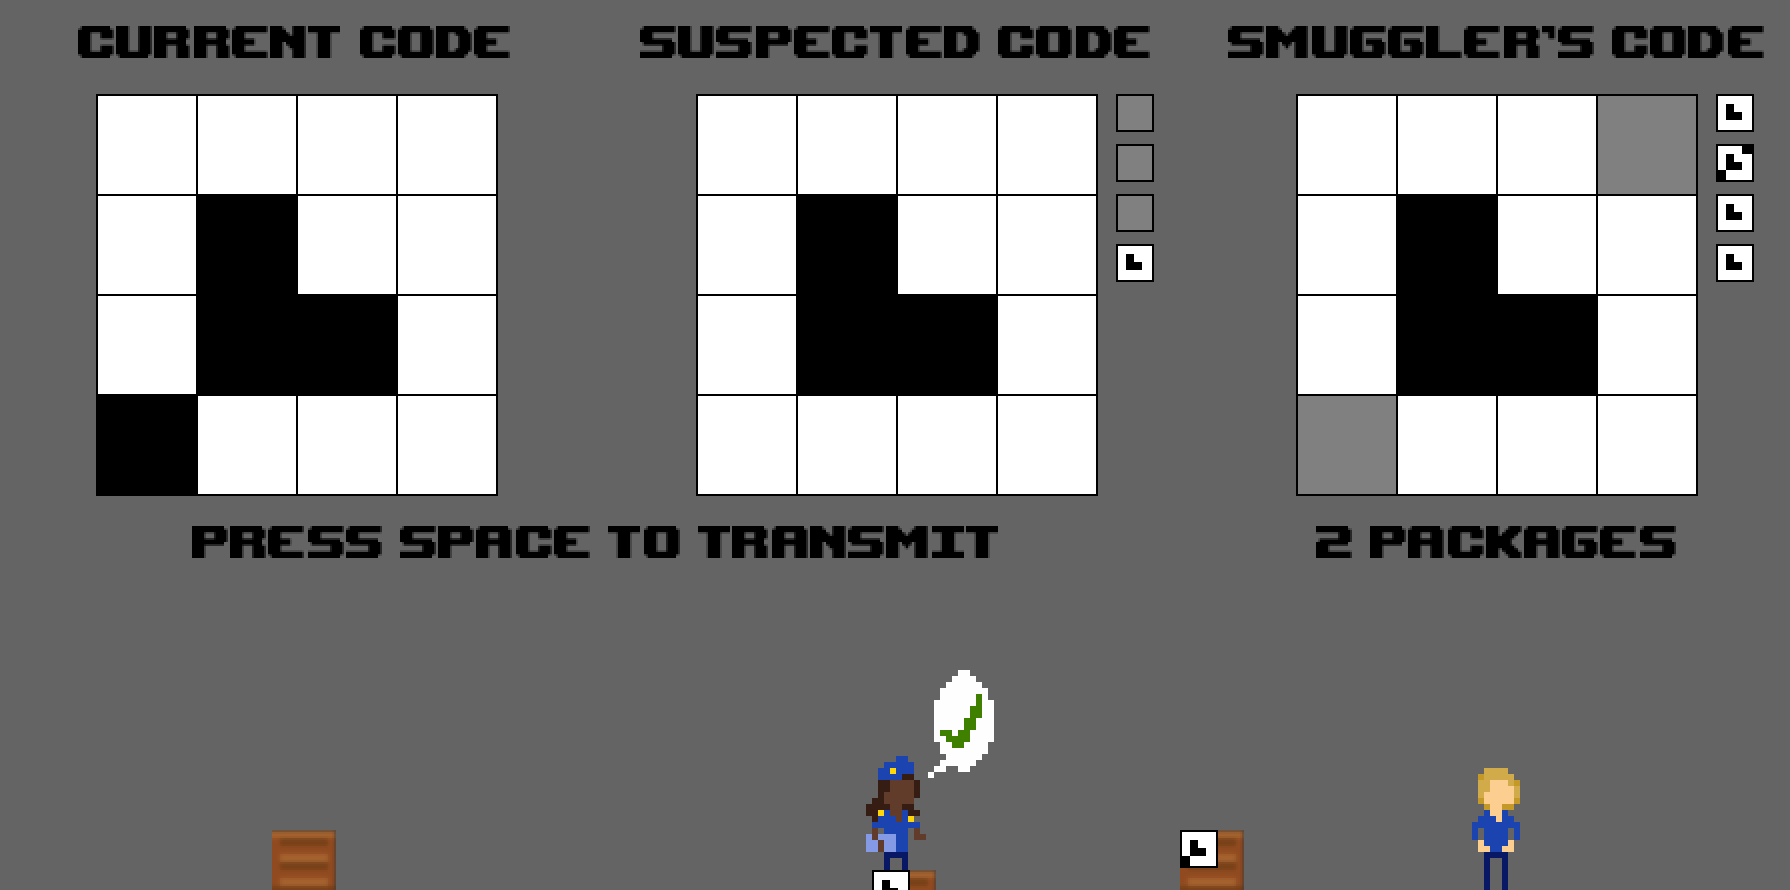
\includegraphics[width=\textwidth]{contrabot}
%\caption{\label{fig:contrabot}A screenshot of~\textit{Contrabot}, which was built from scratch in one evening in an informal game jam.
%The game was built by five of the members of the `AI-Based Game Design' working group at Dagstuhl seminar 15051: Artificial and Computational Intelligence and Games.}
%\end{figure}

\textit{Contrabot} illustrates how to adopt a specific AI-based game design pattern and expresses the concepts and theories of the discussion group.
Our development experience encouraged scholarly discussion as we worked through design issues in representing an AI algorithm to the player while creating engaging gameplay.
We also needed to address common challenges in team work including code source control, creating art assets, and visual design---all topics beyond the purview of traditional `academic' roles in implementing a learning algorithm (and possibly game logic).
Our experiences developing \textit{Contrabot} furthered discussions on how learning algorithms can be taught (and tricked) and how AI learning provides gameplay opportunities for players.

\newpage

%In addition, it acts as an example of how conducting a game jam during an academic event can reinforce scholarly discussion and research.
%\textit{Contrabot} helped validate the ideas of the group and contributed towards subsequent discussion.
%Furthermore, it is important to acknowledge it was built within less than six hours and in doing so reinforced concepts that, a day prior, were merely conjecture.
%
%Furthermore, while each academic contributed to the games design, each also provided specific skills throughout the games creation.
%This ranged from writing the NPC's learning algorithm and overall game logic to the sprites and user interface.
%While typically the design and implementation of the learning algorithm is typically the role of academics, it is valuable to acknowledge the range of skills within the group. 


%%%%%%%%%%%%%%%%%%%%%%%%%%%%%%%%%%%%%%%%%%%%%%%%%%%%%%

\subsection{Game Jam \#2: What Did You Do?}
The second jam game, \textit{What Did You Do?}, emerged from further discussion among the group about AI-based game design that followed from the work on~\textit{Contrabot}.
%We would argue that the consensus to work on this game emerged largely from the contributions that~\textit{Contrabot} had brought to the discussion.
%
%\begin{figure}[tb]
%\centering
%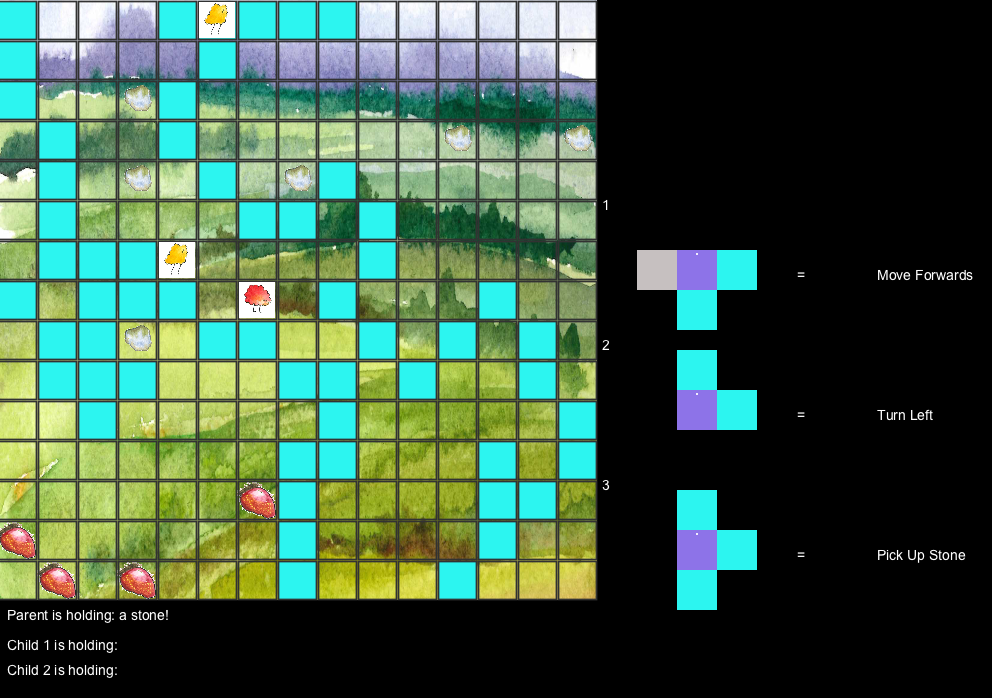
\includegraphics[width=0.5\textwidth]{WDYD}
%\caption{\label{fig:WDYD}A screenshot of~\textit{What Did You Do?}, a game where the player must supervise non-player characters whose behaviours develop as a result of observing the actions of the player.
%The grid pane shows the location of the player and child `shrubs', with the right pane showing the knowledge base the children have learned over time.}
%\end{figure}
%
%The game, as shown in Figure~\ref{fig:WDYD}, tasks the player with ensuring the survival and development of NPC's who are, according to the story, the children of the player.
%As the player begins to explore the world - a grid of land and water tiles - each action they execute is processed by the children, with the possibility that they form into rules.
%During each turn of the game, where the player has the option to act, each child will also make moves with respect to their established rules.
%This ranges not only from movement around the environment where actions are taken relative to their local surroundings (e.g. `If water is to my left, walk forward') but also children may pick up rocks lying in the world that the parent would use to traverse routes blocked by water.
%This presents a conundrum for the player, given that the children have the potential to drown in the river or hurt themselves by attempting to carry the rock.
%As such, players have the option of collecting strawberries that, when given to a child, allow the player to remove an established rule.
%As a result, the player must balance between achieving their objective as well as managing the often unpredictable children.
%
We \textit{What Did You Do?} developed with contributions by other members of the AI-based game design work group~\cite{treanor2015:ai-based-game}\footnote{The source code for this project is available at:\url{http://github.com/gamesbyangelina/whatareyoudoing}}.
This project was larger and longer: incorporating a larger team and spanning several evenings and the hackathon day during the seminar.
Many academics worked together a wider range of features including hand-drawn art, voice recording, and controller input.
In contrast to \textit{Contrabot} there was longer formative discussion on the design of \textit{What Did You Do?} with substantial feature planning.

Ultimately, we did not implement all of the desired functionality during the hackathon.
While a failure in achieving the design goals, this resulted in continued collaboration after the seminar ended: with discussion of how best to complete the game and what contributions could still be made to the project.
What started as another opportunity to highlight AI-driven game design, resulted in ongoing collaboration among academics that reinforces the original discussion and produces tangible artifacts to share with the community.
The game demonstrated to Dagstuhl attendees resulted from pragmatic feature-cutting: a valuable experience echoed by game developers\footnote{http://makegames.tumblr.com/post/4061040007/the-full-spelunky-on-spelunky} as an integral part of getting something finished, and a valuable lesson researchers rarely have.

%%%%%%%%%%%%%%%%%%%%%%%%%%%%%%%%%%%%%%%%%%%%%%%%%%%%%%

\section{Recommendations}
Based on our experiences we provide recommendations for including a game jam or hackathon in an academic context.
%We encourage future experiments with this format and research on its effects.

\pseudosection{Advertise game jams as an optional activity.} Game jams should be presented to attendees similarly to workshops: a separate activity taking place on site during the main event that attendees can join should they feel inclined.

\pseudosection{Encourage open collaboration.} Team formation should be free-form, with no set size or structure to group demographics.
This promotes an environment that allows professionals and scholars at all levels (from student to tenured professor) to work together in a welcoming environment.
%\mytodo{reference other inclusivity groups? GS: I think the solution is actually to change the pseudosection header. "inclusivity" justifiably brings to mind questions of gender and racial diversity, not "won't someone please think of the tenured faculty?" :) changed from "favor inclusivity" to "encourage open collaboration"}
	
\pseudosection{Provide physical space.} Provide a open space to allow a variety of working arrangements among contributors, with power and internet access.
This allows groups to form in the event they wish to focus on particular activities.

%\mytodo{[AZ] feels more about hackatons in general, rather than unique to academics}\mytodo{[T2] that's true, but given academics don't hold hackathons, this might need to be clearly stated}
	
\pseudosection{Use time frames instead of deadlines.} A block of time should be set for the jam, with an (optional) opportunity to showcase work.
This can either be within the jamming community or at a presentation session during the main event (the tactic adopted in Schloss Dagstuhl 15051).
	
\pseudosection{Focus on goals.} Participants should focus on the elements of their intended product that are relevant to the original concept.
This may result in artifacts that lack polish or refinement, but these issues can be resolved after the jam has been completed.
While difficult to institute from an organizational perspective, we hope this ethic will grow as more academic events incorporate jams and academics are exposed to the format.
%\mytodo{[AZ] feels more about hackatons in general, rather than unique to academics}
	
%	\item[Reflect on what is achieved, not what was missed] A jam is a tremendous opportunity to craft a simple prototype of your ideas.
%	It is neither expected to be completed, or work well.
%	The value comes from that which is learned during the process.
%	\mytodo{[AZ] good general advice but maybe not specific to jams}

\pseudosection{Encourage post-jam development.} In many cases, these projects can be expanded upon in the future should the team continue to be enthusiastic towards them.


\section{Challenges}
%\mytodo{AZ: any way to flesh this out to balance?}
%
%\mytodo{T2: Not really sure what arguments can be made here or advice can be given, since this has not really been adopted in conference organisation as yet.}
%
%\mytodo{I don't know if this is wanted/needed but here's some stuff off the top of my head that might be good to head off reviewer criticism or concern. We could work this into other areas or just remove it outright? - MC}
%\mytodo{[AZ] think this can fold into the recommendations by rephrasing a bit, e.g. ``Resources'' could become something like `Provide Resources'}
Incorporating game jams into academic events involves overcoming challenges in the time needed for the event and resources required for game development.

\pseudosection{Time Consumption.} Game jams are often time constrained, with a typical length of 48 hours where many entrants work for 30-40 hours.
Academic events are often time-constrained as attendees may have traveled long distances and only for a few days.
Dagstuhl offered ample time to work, but even half a day in a conference schedule is a small time window to produce games in (and replaces up to a dozen potential talk slots).

We believe this may require a shift in the hackathon culture for such events, where the scheduled time is seen as a `kickoff' phase, with projects continued in social hours throughout the event.
Additionally, many jams take place in much smaller time frames, such as the 0-Hour Game Jam\footnote{http://0hgame.eu/}---they simply require a different approach and different prioritization, something which can be worked on and developed through future hackademic events.

\pseudosection{Resources.} Game jams thrive on collaboration between differently skilled individuals, however academic events tend to collect people with similar skills from a game development standpoint (the interdisciplinary benefit comes from their varied academic backgrounds).
This means that groups without artists, musicians or designers will be common at many events---we were fortunate at Dagstuhl to be assisted by an artist who produced assets for~\textit{What Did You Do?}

Game jam entries do not need art or music, but they can make people feel easier about sharing and presenting their work.
This problem can be mitigated by increasing the awareness of free resources such as Incompetech\footnote{http://incompetech.com/} or Open Game Art\footnote{http://opengameart.org/}.
Providing resources in advance can boost confidence and overcome apprehension in people new to jamming.


%%%%%%%%%%%%%%%%%%%%%%%%%%%%%%%%%%%%%%%%%%%%%%%%%%%%%%

\section{Conclusions}
This paper provides an argument for the inclusion of games jam and `hackathon' events as part of the program and ethos of games-driven academic conferences.
We argue for the relevance and value of these activities within existing academic conferences, with examples of successful practice and recommendations for how to provide similar activities for organizational committees to consider.

Game jams can provide real intellectual currency and enhance our discussions of research problems that are still not yet fully formulated or otherwise established.
Jams also offer wide-ranging individual benefits: personal growth through collaboration, developing research prototypes, and gaining game development experience relevant to pedagogy.
In addition to fostering creativity, encouraging open collaboration and potential inter-disciplinary research it is important to recall above all else: game jams are fun!

% What do you think?  Too much? - T2

%%%%%%%%%%%%%%%%%%%%%%%%%%%%%%%%%%%%%%%%%%%%%%%%%%%%%%

%ACKNOWLEDGMENTS are optional
\section{Acknowledgments}
The authors wish to acknowledge Adam Smith from the~\textit{Contrabot} team, as well as Mirjam Eladhari and Antonios Liapis for their contributions to~\textit{What Did You Do?}
This paper is a direct result of collaborations begun at Schloss Dagstuhl seminar 15051 in January 2015.  The authors thank the Dagstuhl organizers and staff for their support.

%Bibliography
\bibliographystyle{abbrv}
\bibliography{lib}

%\balancecolumns
\end{document}